\begin{figure}[h!]
    \centering
    \caption{Association between Police Resources and Police Effectiveness in Municipalities implementing \emph{Plan Cuadrante} before 2006 and never treated municipalities (Post-\emph{Plan Cuadrante} Period)}
    \label{fig:figureA7}
    \begin{subfigure}{0.45\textwidth}
        \centering
        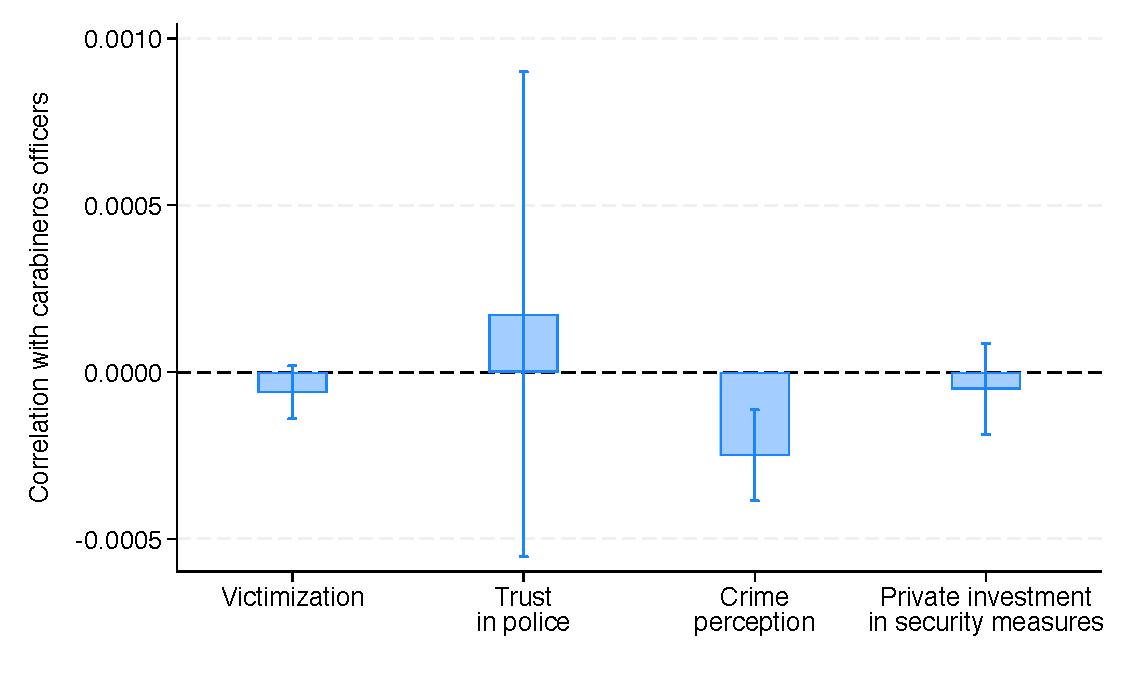
\includegraphics[width=\textwidth]{../manuscript/Graphs/results_carabineros_corr_novariation_enusc.pdf}
                \caption{Victimization and Security Perception \\ by Increase in Police Officers}
    \end{subfigure}
    ~
    \begin{subfigure}{0.45\textwidth}
        \centering
        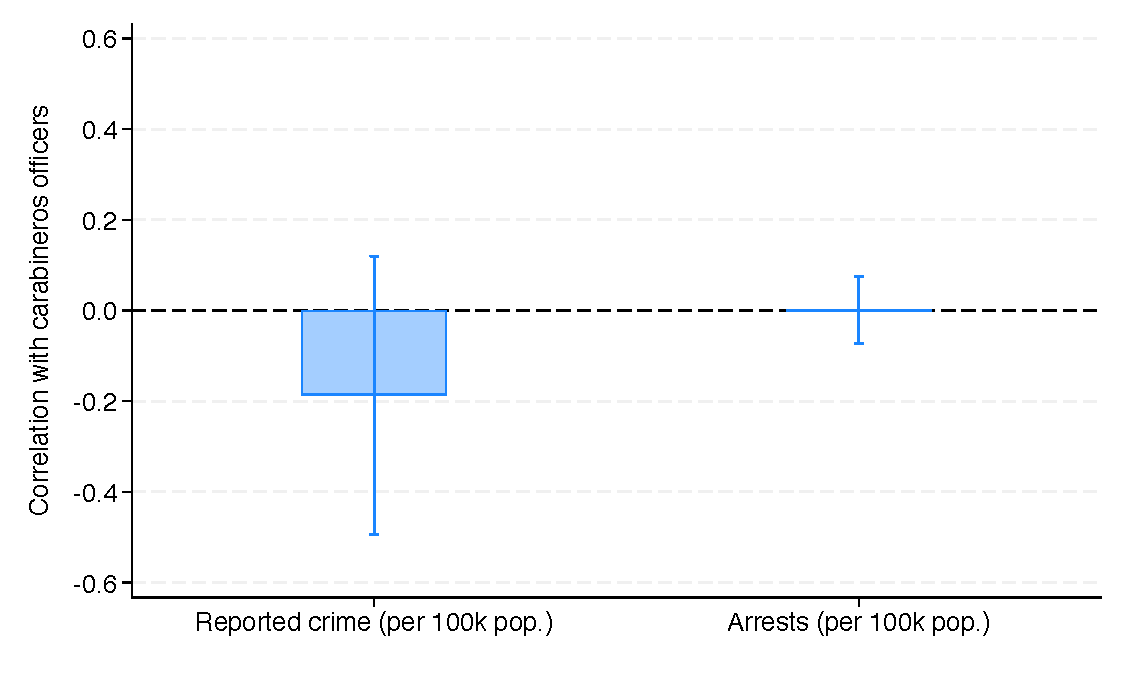
\includegraphics[width=\textwidth]{../manuscript/Graphs/results_carabineros_corr_novariation_spd.pdf}
                \caption{Reported crime and Arrests\\ by Increase in Police Officers}
    \end{subfigure}
     \begin{subfigure}{0.45\textwidth}
        \centering
        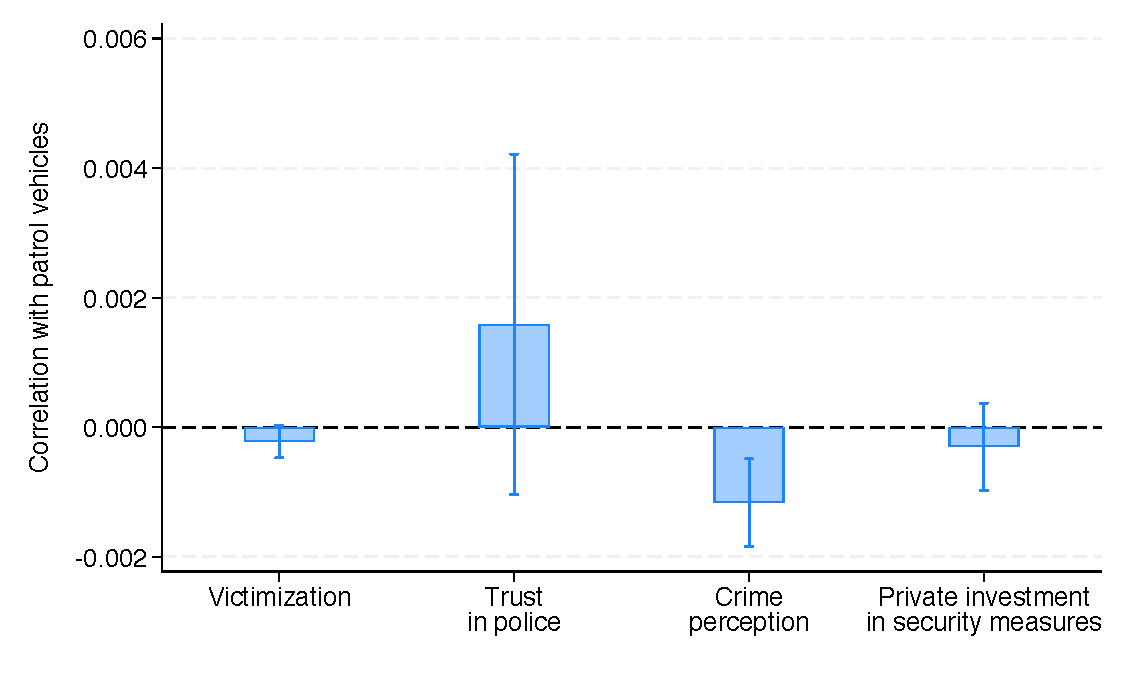
\includegraphics[width=\textwidth]{../manuscript/Graphs/results_vehicles_corr_novariation_enusc.pdf}
                \caption{Victimization and Security Perception \\ by Increase in Patrol Vehicles}
    \end{subfigure}
    ~
    \begin{subfigure}{0.45\textwidth}
        \centering
        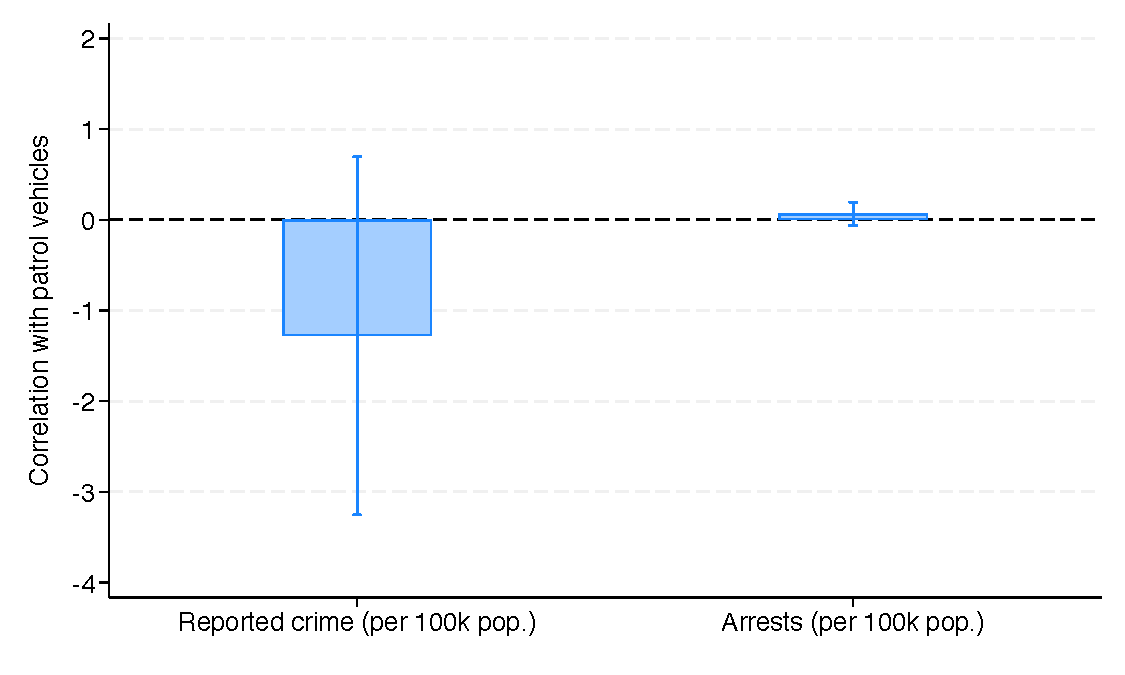
\includegraphics[width=\textwidth]{../manuscript/Graphs/results_vehicles_corr_novariation_spd.pdf}
                \caption{Reported crime and Arrests\\ by Increase in Patrol Vehicles}
    \end{subfigure}
    \\[12pt]
    \begin{minipage}{0.99\textwidth}
    \footnotesize Notes: The figure shows the statistical association between police resources and the main outcomes. The analysis is conducted for the 62 municipalities that introduced \emph{Plan Cuadrante} before 2006 and the never treated municipalities surveyed in ENUSC for the period 2006-2012. The estimation is conducted using OLS with municipality and year fixed effects. The graphs show the estimated coefficients and 95\% confidence intervals. Standard errors are clustered at the municipality level using the wild bootstrapping procedure. Panel (a) reports the association between the number of police officers and the victimization and security perception outcomes included in the ENUSC survey. Panel (b) reports the association between the number of police officers and the outcomes constructed using the administrative information on arrests and crimes reported to the police provided by the Undersecretary for Crime Prevention. Panel (c) reports the association between the number of patrol vehicles and the victimization and security perception outcomes included in the ENUSC survey. Panel (d) reports the association between the number of patrol vehicles and the number of police officers and the outcomes constructed using the administrative information on arrests and crimes reported to the police provided by the Undersecretary for Crime Prevention. 
    \end{minipage}
\end{figure}

